%-----------------------------------------------------------------------------------------------------------------------------------------------%
%	The MIT License (MIT)
%
%	Copyright (c) 2016 Jan Küster
%
%	Permission is hereby granted, free of charge, to any person obtaining a copy
%	of this software and associated documentation files (the "Software"), to deal
%	in the Software without restriction, including without limitation the rights
%	to use, copy, modify, merge, publish, distribute, sublicense, and/or sell
%	copies of the Software, and to permit persons to whom the Software is
%	furnished to do so, subject to the following conditions:
%	
%	THE SOFTWARE IS PROVIDED "AS IS", WITHOUT WARRANTY OF ANY KIND, EXPRESS OR
%	IMPLIED, INCLUDING BUT NOT LIMITED TO THE WARRANTIES OF MERCHANTABILITY,
%	FITNESS FOR A PARTICULAR PURPOSE AND NONINFRINGEMENT. IN NO EVENT SHALL THE
%	AUTHORS OR COPYRIGHT HOLDERS BE LIABLE FOR ANY CLAIM, DAMAGES OR OTHER
%	LIABILITY, WHETHER IN AN ACTION OF CONTRACT, TORT OR OTHERWISE, ARISING FROM,
%	OUT OF OR IN CONNECTION WITH THE SOFTWARE OR THE USE OR OTHER DEALINGS IN
%	THE SOFTWARE.
%
%	RESOURCES USED:
%	http://tex.stackexchange.com/questions/5718/package-for-pie-charts
%	http://tex.stackexchange.com/questions/183087/draw-colored-world-us-map-in-latex#183138
%	http://www.texample.net/tikz/examples/simple-flow-chart/
%	http://vizualize.me/#
%-----------------------------------------------------------------------------------------------------------------------------------------------%


%============================================================================%
%
%	DOCUMENT DEFINITION
%
%============================================================================%

%we use article class because we want to fully customize the page
\documentclass[10pt,A4]{article}	


%----------------------------------------------------------------------------------------
%	ENCODING
%----------------------------------------------------------------------------------------

%we use utf8 since we want to build from any machine
\usepackage[utf8]{inputenc}		

%----------------------------------------------------------------------------------------
%	LOGIC
%----------------------------------------------------------------------------------------

% provides \isempty test
\usepackage{xifthen}
\usepackage{calc}

%----------------------------------------------------------------------------------------
%	FONT
%----------------------------------------------------------------------------------------

% some tex-live fonts - choose your own

%\usepackage[defaultsans]{droidsans}
%\usepackage[default]{comfortaa}
%\usepackage{cmbright}
\usepackage[default]{raleway}
%\usepackage{fetamont}
%\usepackage[default]{gillius}
%\usepackage[light,math]{iwona}
%\usepackage[thin]{roboto} 

% set font default
\renewcommand*\familydefault{\sfdefault} 	
\usepackage[T1]{fontenc}

% more font size definitions
\usepackage{moresize}		


%----------------------------------------------------------------------------------------
%	PAGE LAYOUT  DEFINITIONS
%----------------------------------------------------------------------------------------

%debug page outer frames
%\usepackage{showframe}			


%define page styles using geometry
\usepackage[a4paper]{geometry}		

% for example, change the margins to 2 inches all round
\geometry{top=1.75cm, bottom=-.6cm, left=1.5cm, right=1.5cm} 	


%use customized header
\usepackage{fancyhdr}				
\pagestyle{fancy}

%less space between header and content
\setlength{\headheight}{-5pt}		


%customize entries left, center and right
\lhead{}
\rhead{}

\setlength{\parindent}{0mm}	%indentation is zero

%----------------------------------------------------------------------------------------
%	TABLE /ARRAY DEFINITIONS
%---------------------------------------------------------------------------------------- 

\usepackage{multicol}			
\usepackage{multirow}

\usepackage{array}	%extended aligning of tabular cells

\newcolumntype{x}[1]{%
>{\raggedleft\hspace{0pt}}p{#1}}%


%----------------------------------------------------------------------------------------
%	GRAPHICS DEFINITIONS
%---------------------------------------------------------------------------------------- 

\usepackage{graphicx}	%for header image
\usepackage{wrapfig}	%for floating figures
\usepackage{float}
%\floatstyle{boxed} 
%\restylefloat{figure}

		
\usepackage{tikz}	%for drawing graphics
\usetikzlibrary{shapes, backgrounds}

\newcommand{\icons}{Font-Awesome-SVG-PNG/white/png/64/}	%path to your icon lib
\newcommand{\icon}[2]{\includegraphics[height=#2]{\icons#1}}	%icon shortcut
\newcommand{\icontext}[3]{ 						%icon with text shortcut
	\mbox{
		\icon{#1}{#2} #3
	}
}

%----------------------------------------------------------------------------------------
%	Color DEFINITIONS
%---------------------------------------------------------------------------------------- 

\usepackage{color}

%accent color
\definecolor{sectcol}{RGB}{255,150,0}

\definecolor{secondcol}{RGB}{50,50,255}

%dark background color
\definecolor{bgcol}{RGB}{110,110,110}

%light background / accent color
\definecolor{softcol}{RGB}{225,225,225}

%background col for whole page
\pagecolor{bgcol}

%============================================================================%
%
%
%	DEFINITIONS
%
%
%============================================================================%

%----------------------------------------------------------------------------------------
% 	HEADER
%----------------------------------------------------------------------------------------

% remove top header line
\renewcommand{\headrulewidth}{0pt} 

%remove botttom header line
\renewcommand{\footrulewidth}{0pt}	  	

%remove pagenum
\renewcommand{\thepage}{}	

%remove section num		
\renewcommand{\thesection}{}			

\chead{ \small{Bremen, Germany  $\cdot$  \textcolor{sectcol}{\textbf{info@jankuester.com}} $\cdot$ +49 176 313 877 34}}

%----------------------------------------------------------------------------------------
% 	ARROW GRAPHICS in Tikz
%----------------------------------------------------------------------------------------

% a six pointed arrow poiting to the left
\newcommand{\tzlarrow}{(0,0) -- (0.2,0) -- (0.3,0.2) -- (0.2,0.4) -- (0,0.4) -- (0.1,0.2) -- cycle;}	

% a six pointed arrow poiting to the right
\newcommand{\tzrarrow}{ (0,0.2) -- (0.1,0) -- (0.3,0) -- (0.2,0.2) -- (0.3,0.4) -- (0.1,0.4) -- cycle;}


% include the left arrow into a tikz picture
% param1: fill color
%
\newcommand{\larrow}[1]
{\begin{tikzpicture}[scale=0.58]
	 \filldraw[fill=#1!100,draw=#1!100!black]  \tzlarrow
 \end{tikzpicture}
}

% include the right arrow into a tikz picture
% param1: fill color
%
\newcommand{\rarrow}[1]
{\begin{tikzpicture}[scale=0.58]
	\filldraw[fill=#1!100,draw=#1!100!black] \tzrarrow
 \end{tikzpicture}
}


% draw a slice for a chart
% param 1:
% param 2:
% param 3:
% param 4:
% param 5:
% param 6:
\newcommand{\slice}[6] {
 	\pgfmathparse{0.5*#1+0.5*#2}
  	\let\midangle\pgfmathresult
 	
	% slice
  	\filldraw[fill=#5!100,draw=bgcol!100, line width=2.5pt,  inner sep=15pt ] (0,0) -- (#1:#6) arc (#1:#2:#6) -- cycle;

  	% outer label
  	\node[label=\midangle:\textcolor{white}{#4}] at (\midangle:#6) {};
}

%counters for chart loop
\newcounter{a}
\newcounter{b}
\newcounter{c}

% draws a pie chart by a list of input values
% param 1: the value list ->example: 20/type A, 4/type B, 11/type C, 49/type D, 16/other
% param 2: scaling factor (no font scaling)
% param 3: circle size, use 90, 180, 270 or 360
% param 4: caption
\newcommand{\chart}[4]{
	%reset counters
	\setcounter{a}{0}
	\setcounter{b}{0}
	\setcounter{c}{50}
	\begin{tikzpicture}[scale=3]
	\foreach \p/\t in {#1} {
		\setcounter{a}{\value{b}}
	    	\addtocounter{b}{\p}
		\addtocounter{c}{35}
		\definecolor{currentcolor}{RGB}{255, \thec, 0}
	    	\slice{\thea/100*#3}{\theb/100*#3}{\p\%}{\t}{currentcolor}{#2}
	}
	\node[label=#4] at (0,-0.25) {};	%caption
	\end{tikzpicture}\\
}

\newcommand{\bubble}[5]{ 	
	% slice
  	%\filldraw[fill=sectcol!100,draw=none ] ellipse (20:20);

  	% outer label
  	%\node[label=\midangle:\textcolor{white}{#4}] at (\midangle:#6) {};
}

\newcommand{\bubbles}[1]{
	%reset counters
	\setcounter{a}{0}
	\setcounter{b}{0}
	\setcounter{c}{50}
	\begin{tikzpicture}[scale=3]
	\foreach \p/\t in {#1} {
		\setcounter{a}{\value{b}}
	    	\addtocounter{b}{\p}
		\definecolor{currentcolor}{RGB}{255, \thec, 0}
	    	\bubble{\thea}{\theb}{\p}{\t}{currentcolor}
	}
	\end{tikzpicture}
}

%----------------------------------------------------------------------------------------
%	social info
%----------------------------------------------------------------------------------------



%----------------------------------------------------------------------------------------
%	custom sections
%----------------------------------------------------------------------------------------

% create a coloured box with arrow and title as cv section headline
% param 1: section title
%
\newcommand{\cvsection}[1] {
	\rarrow{sectcol} \textcolor{white}{\textbf{#1}}  \larrow{sectcol}
}

%create a coloured arrow with title as cv meta section section
% param 1: meta section title
%
\newcommand{\metasection}[2] {
	\begin{tabular*}{1\textwidth}{p{2.4cm} p{11cm}}
		\larrow{bgcol}	\normalsize{\textcolor{sectcol}{#1}}&#2\\[12pt]
	\end{tabular*}
}

%----------------------------------------------------------------------------------------
%	 CV EVENT
%----------------------------------------------------------------------------------------

% creates a stretched box as cv entry headline followed by two paragraphs about 
% the work you did
% param 1:	event time i.e. 2014 or 2011-2014 etc.
% param 2:	event name (what did you do?)
% param 3:	institution (where did you work / study)
% param 4:	what was your position
% param 5:	some words about your contributions
%
\newcommand{\cvevent}[5]
{
\vspace{8pt}
	\begin{tabular*}{1\textwidth}{p{2.3cm}  p{10.8cm} x{3.9cm}}
 \textcolor{bgcol}{#1}& \textbf{#2} & \vspace{2.5pt}\textcolor{sectcol}{#3}

	\end{tabular*}
\vspace{-12pt}
\textcolor{softcol}{\hrule}
\vspace{6pt}
	\begin{tabular*}{1\textwidth}{p{2.3cm} p{14.4cm}}
&		 \larrow{bgcol}  #4\\[3pt]
&		 \larrow{bgcol}  #5\\[6pt]
	\end{tabular*}

}

% creates a stretched box as 
\newcommand{\cveventmeta}[2]
{
	\mbox{\mystrut \hspace{87pt}\textit{#1}}\\
	#2
}

%----------------------------------------------------------------------------------------
% CUSTOM STRUT FOR EMPTY BOXES
%----------------------------------------- -----------------------------------------------
\newcommand{\mystrut}{\rule[-.3\baselineskip]{0pt}{\baselineskip}}

%----------------------------------------------------------------------------------------
% CUSTOM LOREM IPSUM
%----------------------------------------------------------------------------------------
\newcommand{\lorem}{Lorem ipsum dolor sit amet, consectetur adipiscing elit. Donec a diam lectus.}


%============================================================================%
%
%
%
%	DOCUMENT CONTENT
%
%
%
%============================================================================%
\begin{document}


%use our custom fancy header definitions
\pagestyle{fancy}	


%---------------------------------------------------------------------------------------
%	TITLE HEADLINE
%----------------------------------------------------------------------------------------

\begin{center}
\HUGE{\textcolor{white}{\textsc{Jan Küster}} }\\[-30pt]
\textcolor{sectcol}{\hrule}
\vspace{5pt}
\Large{\textcolor{white}{\textsc{Software Engineer and Consultant}}}\\
\end{center}

\small


%---------------------------------------------------------------------------------------
%	QR CODE (optional)
%----------------------------------------------------------------------------------------
%\vspace{-136pt}
%\hspace{0.75\linewidth}
%
\includegraphics[width=103pt]{qrcode}
%\normalsize
%\vspace{88pt}

%---------------------------------------------------------------------------------------
%	META SECTION
%----------------------------------------------------------------------------------------

%\vspace{-114pt}


\metasection{Status:}{Bremen, Germany}
\metasection{Degree:}{M.Sc. Digital Media}
%\metasection{Activities:}{Global Game Jam, Sound Engineering, Blender, Martial Arts}


\begin{center}
\chart{9/Design, 25/Projects, 25/Consulting,41/Software Dev}{0.85}{180}{\cvsection{Skills}}\bubbles{5/js , 3/java , 3/xpages , 2/latex, 4/as3}
\end{center}

%	js , java , xpages , latex, as3
% 	git, eclipse, meteor,
%	

%---------------------------------------------------------------------------------------
%	SUMMARAY (optional)
%----------------------------------------------------------------------------------------

%\cvsection{Summary}\\
\icontext{android}{32pt}{Android}

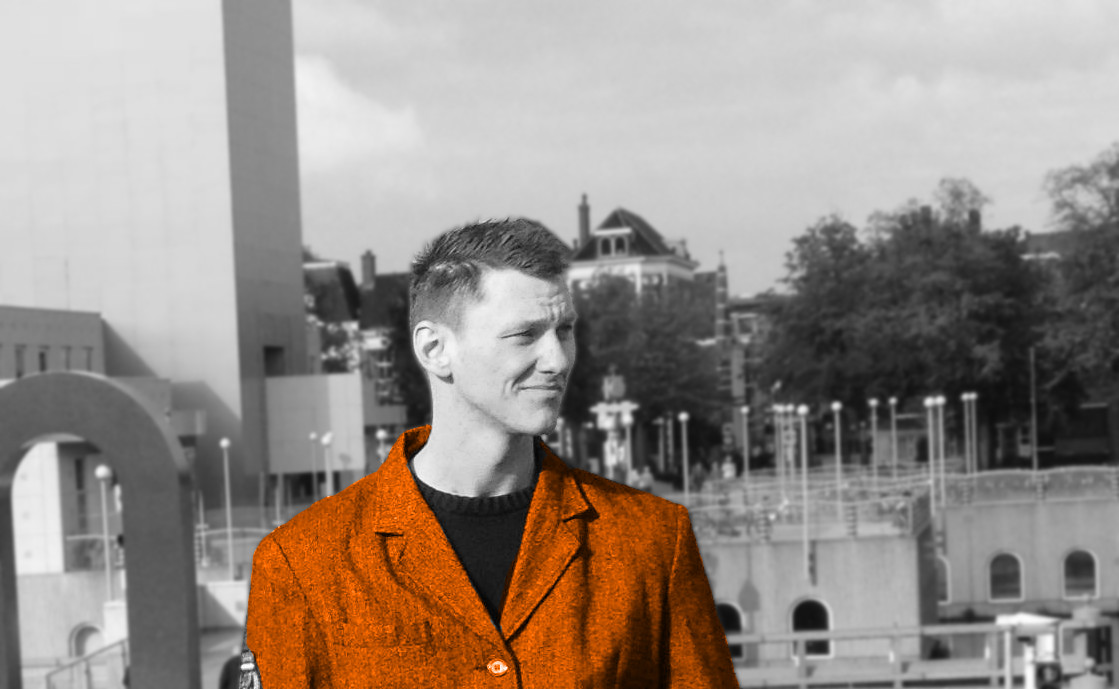
\includegraphics[trim= 320 130 460 210,clip,width=0.2\linewidth]{myfoto.jpg}	%trimming relative to image size!

\newpage
%============================================================================%
%
%	CV SECTIONS AND EVENTS (MAIN CONTENT)
%
%============================================================================%

%---------------------------------------------------------------------------------------
%	EXPERIENCE
%----------------------------------------------------------------------------------------
\cvsection{Experience}

%
\cvevent{2014 - Present}{IT Consultant for IBM XPages and Notes Domino}{We4IT GmbH Bremen}{Realize projects in XPages and We4IT Aveedo, monitor project status, conduct reports}{Implement the frontend for a BPMN compatible engine within We4IT Aveedo}

%\textcolor{softcol}{\hrule}

%
\cvevent{2013 / 09}{Poster Presentation}{DELFI Conference}{Co-published poster with paper on usability guidelines for tests with functional illiterates}{Presented results to conference audience at conference event}

%\textcolor{softcol}{\hrule}

%
\cvevent{2012 - 2014}{Scientific Employee / Software Development}{University of Bremen}{Invented a flexible assessment framework, targeting industrial trainees}{Supervised software development lifecycle, Recruited team members}

%\textcolor{softcol}{\hrule}

%
\cvevent{2011 / 11}{Project Management Simulation Training}{Getoq Consulting}{Performed a two-day project simulation from management perspective}{Topics included customer contracts, change management, controlling, operational tasks}

%\textcolor{softcol}{\hrule}


%
\cvevent{2010 - 2011}{Student Assistant / Programmer}{otulea.uni-bremen.de}{Realized an online diagnosis platform for workforce literacy development (Flex)}{Modeled software design, implemented various prototypes, conducted usability tests}


%---------------------------------------------------------------------------------------
%	EDUCATION SECTION
%--------------------------------------------------------------------------------------
\cvsection{Education}

\cvevent{2015 / 07}{Graduated as M.Sc. Digital Media}{University of Bremen}{Master Thesis: Semi Automated Scoring in Technology Based Assessment}{Developed and evaluated an algorithm for semi automated scoring of spreadsheet data}

%\textcolor{softcol}{\hrule}

%
\cvevent{2012 - 2013}{Master Project - PrIMA}{University of Bremen}{Co-Invented a touch table application for medical support, co-developed software (Java) }{Formed a scrum team, mainted project dev server (Debian), surveyed target audience}

%\textcolor{softcol}{\hrule}

%
\cvevent{2012 - 2015}{Master Studies Digital Media}{University of Bremen}{Inter-cultural classes in English, covering special topics in computer science and design}{Professionalized in research methods, software development and e-assessment}

%\textcolor{softcol}{\hrule}

%
\cvevent{2009 - 2010}{Semester Abroad}{University of Melbourne}{Mastered six months of study and trans-cultural experience in Melbourne, Australia}{Finished machine programming, information visualization, professional essay writing}


%-------------------------------------------------------------------------------------------------
%	ARTIFICIAL FOOTER (fancy footer cannot exceed linewidth) 
%--------------------------------------------------------------------------------------------------

\null
\vspace*{\fill}
\hspace{-0.25\linewidth}\colorbox{bgcol}{\makebox[1.5\linewidth][c]{\mystrut \small \textcolor{white}{www.jankuester.com} $\cdot$ \textcolor{white}{github.com/jankapunkt}}}




%============================================================================%
%
%
%
%	DOCUMENT END
%
%
%
%============================================================================%
\end{document}
